%! TEX program = xelatex

\documentclass{article}
\usepackage[a4paper, margin=3cm]{geometry}
\setlength{\parindent}{0pt}
\setlength{\parskip}{1em}
%\usepackage{fontspec}
%\setmainfont{Lato}

\usepackage{amsmath,amssymb,amsthm}
\usepackage{pgfplots}
\pgfplotsset{compat=1.16}

\title{MATA114 Harjoitus 3}
\author{Mikael Myyrä}
\date{}

\begin{document}
\maketitle

\section*{1.}

\subsection*{(I)}

\[
  \frac{dy}{dx} = xy^2
\]

Tässä funktiolla $g(y) = y^2$ on nollakohta $y = 0$,
joten yhtälöllä on erikoisratkaisu $y \equiv 0$.

Ratkaistaan yleinen ratkaisu separoimalla:
\begin{align*}
  \frac{dy}{dx} &= xy^2 \\
  \frac{1}{y^2}\frac{dy}{dx} &= x \\
  \int \frac{1}{y^2}\,dy &= \int x\,dx \\
  -\frac{1}{y} &= \frac{1}{2}x^2 + C_1, \quad C_1 \in \mathbb{R} \\
  y &= \frac{1}{C - \frac{1}{2}x^2}, \quad C \in \mathbb{R} \\
\end{align*}

Ratkaisukäyriä (C välillä [-1, 1]):

\begin{center}
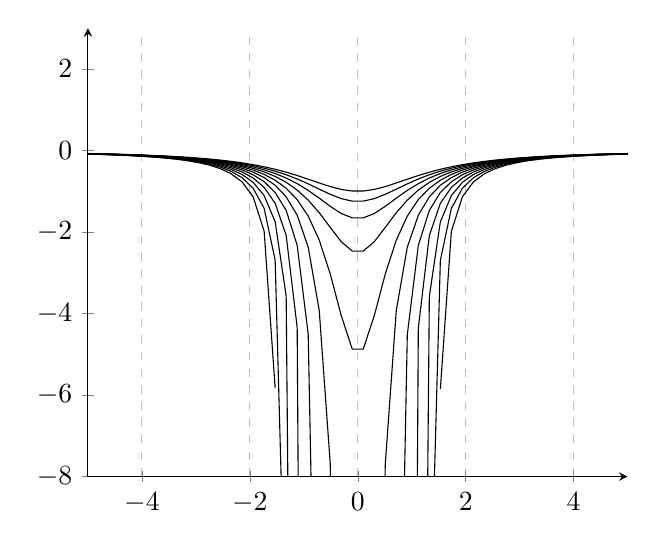
\begin{tikzpicture}
\begin{axis}[
axis lines=left,
grid style=dashed,
xmajorgrids=true,
xmin=-5,
xmax=5,
ymin=-8,
ymax=3,
domain=-5:5,
unbounded coords=jump,
samples=50,
]

\addplot[ ]{(0>=x^2/2?nan:1/(0 - (x^2/2))};
\addplot[ ]{(0.2>=x^2/2?nan:1/(0.2 - (x^2/2))};
\addplot[ ]{(-0.2>=x^2/2?nan:1/(-0.2 - (x^2/2))};
\addplot[ ]{(0.4>=x^2/2?nan:1/(0.4 - (x^2/2))};
\addplot[ ]{(-0.4>=x^2/2?nan:1/(-0.4 - (x^2/2))};
\addplot[ ]{(0.6>=x^2/2?nan:1/(0.6 - (x^2/2))};
\addplot[ ]{(-0.6>=x^2/2?nan:1/(-0.6 - (x^2/2))};
\addplot[ ]{(0.8>=x^2/2?nan:1/(0.8 - (x^2/2))};
\addplot[ ]{(-0.8>=x^2/2?nan:1/(-0.8 - (x^2/2))};
\addplot[ ]{(1>=x^2/2?nan:1/(1 - (x^2/2))};
\addplot[ ]{(-1>=x^2/2?nan:1/(-1 - (x^2/2))};

\end{axis}
\end{tikzpicture}
\end{center}

\subsection*{(II)}

\[
  \frac{dy}{dx} = 2xy(y - 1)
\]

Tässä $g(y) = y(y - 1) = y^2 - y$, jolla on nollakohta $y = 0$.
Siis yhtälöllä on erikoisratkaisu $y \equiv 0$.

Ratkaistaan yleinen ratkaisu:
\begin{align*}
  \frac{dy}{dx} &= 2xy(y - 1) \\
  \frac{1}{y(y - 1)}\frac{dy}{dx} &= 2x \\
  \int \frac{-1}{y} + \frac{1}{y - 1}\,dy &= \int 2x\,dx \\
  -\ln |y| + \ln |y - 1| &= x^2 + C_1, \quad C_1 \in \mathbb{R} \\
  \ln \frac{|y - 1|}{|y|} &= x^2 + C_1 \\
  \frac{|y - 1|}{|y|} &= e^{C_1}e^{x^2} \\
                      &= C_2e^{x^2}, \quad C_2 > 0 \\
  \text{Jos $y \geq 1$ tai $y < 0$:} \\
  \frac{y - 1}{y} &= C_2e^{x^2} \\
  1 - \frac{1}{y} &= C_2e^{x^2} \\
  \frac{1}{y} &= -C_2e^{x^2} + 1 \\
  y &= \frac{1}{-C_2e^{x^2} + 1} \\
    &= \frac{1}{C_3e^{x^2} + 1}, \quad C_3 < 0 \\
  \text{Jos $0 < y < 1$:} \\
  \frac{-y + 1}{y} &= C_2e^{x^2} \\
  y &= \frac{1}{C_2e^{x^2} + 1} \\
\end{align*}

Yhdistämällä nämä saadaan yleinen ratkaisu
\[
  y = \frac{1}{Ce^{x^2} + 1}, \quad C \in \mathbb{R} \setminus \{0\}
\]
tai
\[
  y \equiv 0.
\]

Ratkaisukäyriä (C välillä [-2, 2]):

\begin{center}
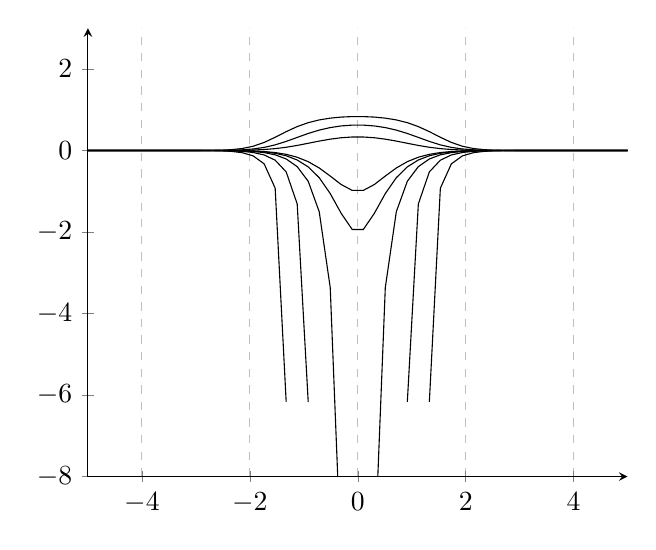
\begin{tikzpicture}
\begin{axis}[
axis lines=left,
grid style=dashed,
xmajorgrids=true,
xmin=-5,
xmax=5,
ymin=-8,
ymax=3,
domain=-5:5,
unbounded coords=jump,
samples=50,
]

\addplot[ ]{(1/(0.2*exp(x^2) + 1))};
\addplot[ ]{(1/(0.6*exp(x^2) + 1))};
\addplot[ ]{(1/(2*exp(x^2) + 1))};
\addplot[ ]{((-0.2*exp(x^2) + 1)>0?nan:1/(-0.2*exp(x^2) + 1))};
\addplot[ ]{((-0.5*exp(x^2) + 1)>0?nan:1/(-0.5*exp(x^2) + 1))};
\addplot[ ]{(1/(-exp(x^2) + 1))};
\addplot[ ]{(1/(-1.5*exp(x^2) + 1))};
\addplot[ ]{(1/(-2*exp(x^2) + 1))};

\end{axis}
\end{tikzpicture}
\end{center}

Käyrät x-akselin alapuolella ovat melko saman muotoisia kuin edellisessä
kohdassa. Molemmat hajaantuvat samalla tavalla kohti $-\infty$:tä, kun
nimittäjän lauseke lähestyy nollaa. Kun nimittäjä on nolla, yhtälössä on
epäjatkuvuuskohta. Eroavaisuutena on, että (II)-kohdassa on koko
$\mathbb{R}$:ssä jatkuvia ratkaisuja myös y-akselin yläpuolella, koska x:n
lausekkeen kerroin saa myös positiivisia arvoja.

\subsection*{Alkuarvotehtävät}

\[
  \begin{cases}
    \frac{dy}{dx} = xy^2 \\
    y(0) = \frac{1}{2} \\
  \end{cases}
\]

Yhtälön ratkaisu on (I)-kohdasta
$y = \frac{1}{C - \frac{1}{2}x^2}, \quad C \in \mathbb{R}$.

Sijoitetaan alkuehto:
\begin{align*}
  \frac{1}{C - \frac{1}{2}0^2} &= \frac{1}{2} \\
  C &= 2 \\
\end{align*}

Saadaan
\[
  y = \frac{1}{2 - \frac{1}{2}x^2}, \quad C \in \mathbb{R}.
\]

Vastaavasti alkuehdolla $y(0) = -\frac{1}{2}$ saadaan
\[
  y = \frac{1}{-2 - \frac{1}{2}x^2}, \quad C \in \mathbb{R}.
\]

Kuvaajat:

\begin{center}
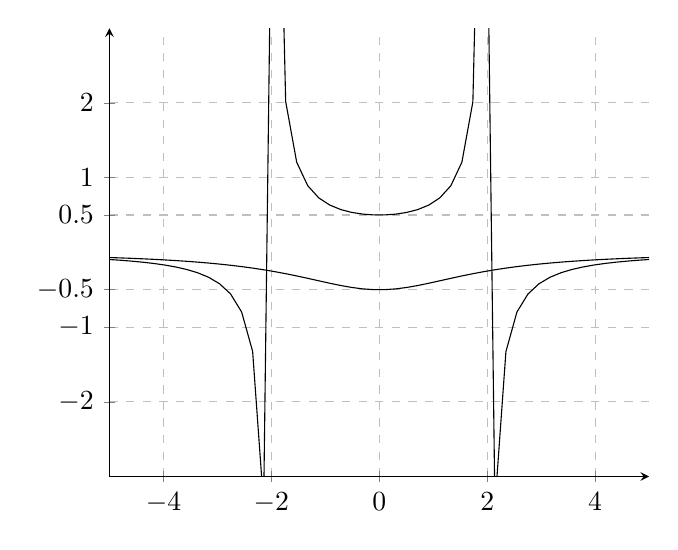
\begin{tikzpicture}
\begin{axis}[
axis lines=left,
grid style=dashed,
xmajorgrids=true,
ymajorgrids=true,
ytick={-2,-1,-0.5,0.5,1,2},
xmin=-5,
xmax=5,
ymin=-3,
ymax=3,
domain=-5:5,
unbounded coords=jump,
samples=50,
]

\addplot[ ]{(1/(2 - (x^2/2))};
\addplot[ ]{(1/(-2 - (x^2/2))};

\end{axis}
\end{tikzpicture}
\end{center}

\section*{2.}

\subsection*{(a)}

\[
  \frac{dy}{dx} = \frac{x^2 + y^2}{2xy}
\]

Jos $x = 0$, niin nimittäjään tulee nolla ja yhtälö ei ole määritelty.
Siis nolla ei kuulu ratkaisuvälille.

\begin{align*}
  \frac{dy}{dx} &= \frac{x^2 + y^2}{2xy} \\
                &= \frac{1 + \frac{y^2}{x^2}}{\frac{2y}{x}} \\
\end{align*}

Muuttujanvaihto: $u = \frac{y}{x}$, $y = xu$, $\frac{dy}{dx} = u + x\frac{du}{dx}$.

\begin{align*}
  u + x\frac{du}{dx} &= \frac{1 + u^2}{2u} \\
  x\frac{du}{dx} &= \frac{1 + u^2}{2u} - u \\
                 &= \frac{1 - u^2}{2u} \\
  \frac{du}{dx} &= \frac{1}{x}(\frac{1 - u^2}{2u}) \\
  \frac{2u}{1 - u^2}\frac{du}{dx} &= \frac{1}{x} \\
  \int\frac{2u}{1 - u^2}\,du &= \int \frac{1}{x}\,dx \\
  -\ln |1 - u^2| &= \ln |x| + C_1, \quad C_1 \in \mathbb{R} \\
  \frac{1}{|1 - u^2|} &= e^{C_1} |x| \\
  |1 - u^2| &= \frac{1}{e^{C_1} |x|} \\
  1 - u^2 &= \pm \frac{1}{e^{C_1} |x|} \\
          &= \frac{1}{C_2 |x|}, \quad C_2 \in \mathbb{R} \setminus \{0\} \\
  u^2 &= 1 - \frac{1}{C_2 |x|} \\
  u &= \pm \sqrt{1 - \frac{1}{C_2 |x|}} \\
\end{align*}

Tästä saadaan $y$ sijoittamalla:
\[
  y = xu = \pm x\sqrt{1 - \frac{1}{C |x|}}, \quad C \in \mathbb{R} \setminus \{0\}
\]

\section*{3.}

\subsection*{(a)}

\begin{align*}
  y(x) &= 2 + \int_0^x \frac{(y(t))^2}{1 + t^2}\,dt \\
  \implies \frac{dy}{dx} &= \frac{(y(x))^2}{1 + x^2} \\
  \text{Jos $y \neq 0$:} \\
  \frac{1}{y^2}\frac{dy}{dx} &= \frac{1}{1 + x^2} \\
  \int \frac{1}{y^2}\,dy &= \int \frac{1}{1 + x^2}\,dx \\
  -\frac{1}{y} &= \arctan x + C, \quad C \in \mathbb{R} \\
  y &= -\frac{1}{\arctan x + C} \\
\end{align*}

Myös $y \equiv 0$ on derivoimalla saadun DY:n ratkaisu.

Integraaliyhtälöstä saadaan lisäksi alkuehto $y(0) = 2$.
\begin{align*}
  -\frac{1}{\arctan 0 + C} &= 2 \\
  -\frac{1}{C} &= 2 \\
  C &= -\frac{1}{2} \\
\end{align*}

Siis yhtälön ratkaisu on
\[
  y = -\frac{1}{\arctan x - \frac{1}{2}}.
\]

\subsection*{(b)}

\begin{align*}
  y(x) &= 3 + \int_0^x e^{-y(t)}\,dt \\
  \implies \frac{dy}{dx} &= e^{-y(x)} \\
  e^y \frac{dy}{dx} &= 1 \\
  \int e^y\,dy &= \int 1\,dx \\
  e^y &= x + C, \quad C \in \mathbb{R} \\
  y &= \ln(x + C) \\
\end{align*}

$e^{-y}$:llä ei ole nollakohtia, joten erikoisratkaisuja ei ole.

Integraaliyhtälöstä alkuehto $y(0) = 3$.
\begin{align*}
  \ln(0 + C) &= 3 \\
  C &= e^3 \\
\end{align*}

Siis yhtälön ratkaisu on
\[
  y = \ln(x + e^3).
\]

\subsection*{(c)}

\begin{align*}
  y(x) &= 2 + \int_1^x (y(t))^2\,dt \\
  \implies \frac{dy}{dx} &= (y(x))^2 \\
  \text{Jos $y^2 \neq 0 \iff y \neq 0$:} \\
  \frac{1}{y^2}\frac{dy}{dx} &= 1 \\
  \int \frac{1}{y^2}\,dy &= \int 1\,dx \\
  -\frac{1}{y} &= x + C, \quad C \in \mathbb{R} \\
  y &= -\frac{1}{x + C} \\
\end{align*}

Myös $y \equiv 0$ on derivoimalla saadun DY:n ratkaisu.

Alkuehto $y(1) = 2$:
\begin{align*}
  -\frac{1}{1 + C} &= 2 \\
  1 + C &= -\frac{1}{2} \\
  C &= -\frac{3}{2}
\end{align*}

Siis yhtälön ratkaisu on
\[
  y = -\frac{1}{x - \frac{3}{2}}.
\]

\section*{4.}

\begin{align*}
  x^2\frac{dy}{dx} + 2xy - y^3 &= 0
  x^2\frac{dy}{dx} + 2xy &= y^3 \\
  \frac{dy}{dx} + \frac{2}{x}y &= \frac{y^3}{x^2} \\
  y^{-3}\frac{dy}{dx} + \frac{2}{x}y^{-2} &= \frac{1}{x^2} \\
\end{align*}

Muuttujanvaihto: $v = y^{-2}$, $\frac{dv}{dx} = -2y^{-3}\frac{dy}{dx}$

\begin{align*}
  y^{-3}\frac{dy}{dx} + \frac{2}{x}y^{-2} &= \frac{1}{x^2} \\
  -\frac{1}{2}\frac{dv}{dx} + \frac{2}{x}v &= \frac{1}{x^2} \\
  \frac{dv}{dx} - \frac{4}{x}v &= -\frac{2}{x^2} \\
\end{align*}
Integroiva tekijä $e^{-4\ln x} = x^{-4}$:
\begin{align*}
  \frac{1}{x^4}(\frac{dv}{dx} - \frac{4}{x}v) &= -\frac{2}{x^6} \\
  \frac{d}{dx}(\frac{1}{x^4}v) &= -\frac{2}{x^6} \\
  \frac{1}{x^4}v &= -\int \frac{2}{x^6}\,dx \\
                 &= \frac{2}{5}x^{-5} + C_1, \quad C_1 \in \mathbb{R} \\
  v &= \frac{2}{5x} + C_1x^4 \\
    &= \frac{2 + 5C_1x^5}{5x} \\
    &= \frac{2 + Cx^5}{5x}, \quad C \in \mathbb{R} \\
\end{align*}

Ratkaistaan $y$:
\begin{align*}
  v &= y^{-2} \\
  y &= \pm \sqrt{v^{-1}} \\
    &= \pm \sqrt{\frac{5x}{2 + Cx^5}} \\
\end{align*}

\section*{5.}

\subsection*{(a)}

\[
  xy^2 + y + (x^2y + x)\frac{dy}{dx} = 0
\]

Yhtälö on muotoa $M(x, y) + N(x, y)\frac{dy}{dx}$,
missä $M = xy^2 + y$ ja $N = x^2y + x$.
Koska $\frac{dM}{dy} = 2xy + 1 = \frac{dN}{dx}$, niin yhtälö on eksakti.

Etsitään ''potentiaalifunktio'' $\phi$, jolle $\frac{d\phi}{dx} = M$ ja
$\frac{d\phi}{dy} = N$:

\begin{align*}
  \frac{d\phi}{dx} &= M = xy^2 + y \\
  \phi &= \int (xy^2 + y)\,dx \\
       &= \frac{1}{2}x^2y^2 + yx + C_1(y) \\
\end{align*}
Etsitään $C_1(y)$ derivoimalla:
\begin{align*}
  \frac{d\phi}{dy} &= x^2y + x + \frac{dC_1}{dy} \\
                   &= N + 0 \\
  \implies \frac{dC_1}{dy} &= 0 \\
  C_1 &= \int 0\,dy = 0 \\
\end{align*}

Siis
\[
  \phi = \frac{1}{2}x^2y^2 + yx
\]
ja DY:n ratkaisu
\[
  \frac{1}{2}x^2y^2 + yx = C, \quad C \in \mathbb{R}.
\]

\section*{6.}

\[
  \frac{dy}{dx} = -xy
\]

\subsection*{(a), (b)}

\includegraphics*[width=300pt]{w3_6.png}

\subsection*{(c)}

\begin{align*}
  \frac{dy}{dx} &= -xy \\
  \text{Jos $y \neq 0$:} \\
  \frac{1}{y}\frac{dy}{dx} &= -x \\
  \int \frac{1}{y}\,dy &= -\int x\,dx \\
  \ln |y| &= -\frac{1}{2}x^2 + C_1, \quad C_1 \in \mathbb{R} \\
  y &= \pm e^{C_1}e^{-\frac{1}{2}x^2} \\
    &= C_2e^{-\frac{1}{2}x^2}, \quad C_2 \in \mathbb{R} \setminus \{0\} \\
\end{align*}

Koska myös $y \equiv 0$ on ratkaisu, niin yleinen ratkaisu on
\[
  y = Ce^{-\frac{1}{2}x^2}, \quad C \in \mathbb{R}.
\]

\subsection*{(d)}

\begin{center}
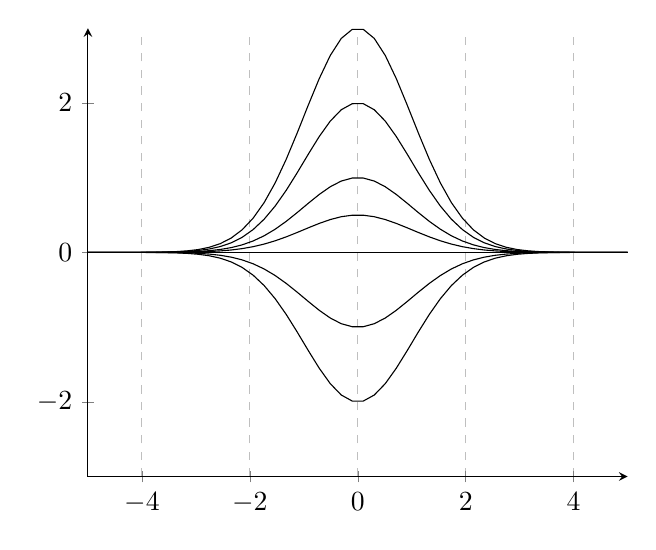
\begin{tikzpicture}
\begin{axis}[
axis lines=left,
grid style=dashed,
xmajorgrids=true,
xmin=-5,
xmax=5,
ymin=-3,
ymax=3,
domain=-5:5,
unbounded coords=jump,
samples=50,
]

\addplot[ ]{(0.5 * exp(-x^2/2)};
\addplot[ ]{(1 * exp(-x^2/2)};
\addplot[ ]{(2 * exp(-x^2/2)};
\addplot[ ]{(3 * exp(-x^2/2)};
\addplot[ ]{(-1 * exp(-x^2/2)};
\addplot[ ]{(-2 * exp(-x^2/2)};
\addplot[ ]{0};

\end{axis}
\end{tikzpicture}
\end{center}

\section*{7.}

\subsection*{(a)}

\[
  \frac{dy}{dx} = \frac{2x}{1 + y^2}
\]

Ratkaistaan DY. Tämä on normaalimuotoinen eksakti DY, jossa $M = -2x$ ja $N = 1
+ y^2$, koska $\frac{dM}{dy} = \frac{dN}{dx} = 0$.  Siis ratkaisu saadaan
etsimällä funktio $\phi$, jolle $\frac{d\phi}{dx} = -2x$ ja $\frac{d\phi}{dy} =
1 + y^2$. Koska $M$ ei riipu lainkaan $y$:stä eikä $N$ $x$:stä, niin voidaan
päätellä, että $\phi$ on integraalien summa:

\begin{align*}
  \phi &= \int M\,dx + \int N\,dy \\
       &= \int (-2x)\,dx + \int (1 + y^2)\,dy \\
       &= -x^2 + y + \frac{1}{3}y^3 \\
\end{align*}
ja siis DY:n ratkaisu on
\[
  \frac{1}{3}y^3 + y - x^2 = C, \quad C \in \mathbb{R}.
\]

Sijoitetaan tähän haluttu piste $(2, 3)$:
\begin{align*}
  \frac{1}{3}*3^3 + 3 - 2^2 &= C \\
  C &= 8 \\
\end{align*}

Saadaan yhtälö
\[
  \frac{1}{3}y^3 + y - x^2 = 8.
\]

Jälkeenpäin ajatellen tässä ei olisi tarvinnut eksaktiutta, vaan samaan
lopputulokseen olisi päässyt kertomalla $(1 + y^2)$:lla ja integroimalla
puolittain.

\subsection*{(b)}

\begin{align*}
  \frac{dy}{dx} &= 1 + \frac{2y}{x} \\
                &= \frac{x + 2y}{x} \\
  -x - 2y + x\frac{dy}{dx} &= 0 \\
\end{align*}

Tämä on muotoa $M + N\frac{dy}{dx} = 0$, mutta ei eksakti. Yritetään palauttaa
eksaktiksi integroivalla tekijällä:
\[
  \frac{\frac{dM}{dy} - \frac{dN}{dx}}{N} = \frac{-2 - 1}{x} = -\frac{3}{x}
\]
Tämä on vain x:stä riippuva funktio, joten tällainen integroiva tekijä on olemassa
ja se on
\[
  \mu = e^{\int (-\frac{3}{x})\,dx} = e^{-3\ln x} = x^{-3}.
\]

Saadaan yhtälö
\[
  -x^{-2} - 2yx^{-3} + x^{-2}\frac{dy}{dx} = 0,
\]
jossa $M = -x^{-2} - 2yx^{-3}$, $N = x^{-2}$ ja $\frac{dM}{dy} = \frac{dN}{dx} = -2x^{-3}$.

Etsitään tälle ''potentiaalifunktio'' $\phi$:
\begin{align*}
  \frac{d\phi}{dx} &= M = -x^{-2} - 2yx^{-3} \\
  \phi &= \int (-x^{-2} - 2yx^{-3})\,dx \\
       &= x^{-1} + yx^{-2} + C(y) \\
  \frac{d\phi}{dy} &= x^{-2} + \frac{dC}{dy} \\
                   &= N + 0 \\
  \implies C(y) &= 0 \\
\end{align*}

Saadaan $\phi = x^{-1} + yx^{-2}$ ja yhtälön ratkaisujoukoksi
\[
  \frac{1}{x} + \frac{y}{x^2} = C.
\]

Sijoitetaan haluttu piste $(1, 3)$:
\begin{align*}
  \frac{1}{1} + \frac{3}{1^2} &= C \\
  C &= 4 \\
\end{align*}

Saadaan yhtälö
\[
  \frac{1}{x} + \frac{y}{x^2} = 4.
\]

\section*{8.}

\[
  \begin{cases}
    \frac{dy}{dx} = xe^{-y} \\
    y(0) = 0 \\
  \end{cases}
\]

Käytin tehtäviin seuraavaa Haskell-skriptiä:
\begin{verbatim}
f :: Float -> Float -> Float
f x y =
  x * exp (-y)

euler :: Float -> Float
euler h =
  step 0.0 0.0
  where
    step x y =
      if x < 2.0 then
        step (x + h) (y + h * f x y)
      else
        y

improvedEuler :: Float -> Float
improvedEuler h =
  step 0.0 0.0
  where
    step x y =
      if x < 2.0 then
        step (x + h) (y + h * (f x y + f (x + h) (y + h * f x y)) / 2.0)
      else
        y

rk4 :: Float -> Float
rk4 h =
  step 0.0 0.0
  where
    step x y =
      if x < 2.0 then
        let
          p = f x y
          q = f (x + h / 2.0) (y + h * p / 2.0)
          r = f (x + h / 2.0) (y + h * q / 2.0)
          s = f (x + h) (y + h * r)
        in step (x + h) (y + h * (p + 2*q + 2*r + s) / 6.0)
      else
        y

main :: IO ()
main = do
  putStrLn (show $ euler 0.2)  -- (a)
  putStrLn (show $ euler 0.1)  -- (b)
  putStrLn (show $ improvedEuler 0.2)  -- (c)
  putStrLn (show $ rk4 0.2)  -- (e)
\end{verbatim}

Skripti tulosti (a)-kohdan vastaukseksi 1.0741599,
(b)-kohtaan 1.0866349, (c)-kohtaan 1.0978973 ja (e)-kohtaan 1.0986137.

\subsection*{(d)}

Ratkaistaan DY.
\begin{align*}
  \frac{dy}{dx} &= xe^{-y} \\
  e^y\frac{dy}{dx} &= x \\
  \int e^y\,dy &= \int x\,dx \\
  e^y &= \frac{1}{2}x^2 + C, \quad C \in \mathbb{R} \\
  y &= \ln (\frac{1}{2}x^2 + C) \\
\end{align*}

Koska $e^{-y}$:llä ei ole nollakohtia, niin erikoisratkaisuja ei ole.
Sijoitetaan alkuehto $y(0) = 0$:
\begin{align*}
  \ln (\frac{1}{2}*0^2 + C) &= 0 \\
  \ln C &= 0 \\
  C &= e^0 = 1 \\
\end{align*}

Siis alkuarvotehtävän ratkaisu on
\[
  y = \ln (\frac{1}{2}x^2 + 1).
\]
Pisteessä $x = 2$ tarkaksi arvoksi saadaan
\[
  y(2) = \ln (\frac{1}{2}2^2 + 1) = \ln 3 \approx 1.0986123.
\]

Siis virhe oli (a)-kohdassa $1.0741599 - 1.0986123 = -0.0244524$,\\
(b)-kohdassa $1.0866349 - 1.0986123 = -0.0119774$,\\
(c)-kohdassa $1.0978973 - 1.0986123 = -0.0007150$\\
ja (e)-kohdassa $1.0986137 - 1.0986123 = 0.0000014$.

\end{document}
